%  LaTeX support: latex@mdpi.com 
%  For support, please attach all files needed for compiling as well as the log file, and specify your operating system, LaTeX version, and LaTeX editor.

%=================================================================
\documentclass[journal,article,submit,moreauthors]{Definitions/mdpi} 
\usepackage{pgfplots}
\pgfplotsset{compat=1.18}
\usetikzlibrary{positioning,shapes.geometric}
%\documentclass[journal,article,submit,moreauthors,unicode]{Definitions/mdpi} % For some letters Palatino lacks
%\documentclass[preprints,article,submit,moreauthors]{Definitions/mdpi} 
%\documentclass[preprints,article,submit,moreauthors,unicode]{Definitions/mdpi} 
% For posting an early version of this manuscript as a preprint, you may use "preprints" as the journal. Changing "submit" to "accept" before posting will remove line numbers.

%--------------------
% Class Options:
%--------------------
%----------
% journal
%----------
% Choose between the following MDPI journals:
% accountaudit, acn, acoustics, actuators, addictions, addictprev, adhesives, adolescents, aee, aerobiology, aeronautics, aerospace, agriculture, agriengineering, agrochemicals, agronomy, ai, aiagents, aichem, aieng, aimater, aimed, aipa, air, aisens, aisoc, algorithms, allergies, alloys, amh, analog, analytica, analytics, anatomia, anesthres, animals, antibiotics, antibodies, antioxidants, applbiosci, appliedchem, appliedmath, appliedphys, applmech, applmicrobiol, applnano, applsci, aps, aquacj, archaeolstud, architecture, arm, arthropoda, asc, asd, asi, astronautics, astronomy, atmosphere, atoms, audiolres, automation, axioms, bacteria, batteries, bcrc, bdcc, beverages, bioactives, biochem, bioengineering, biologics, biology, biomass, biomechanics, biomed, biomedicines, biomedinformatics, biomimetics, biomolecules, biophysica, bioresourbioprod, biosensors, biosphere, biotech, birds, blockchains, bloods, blsf, brainsci, breath, buildings, cancers, carbon, cardio, cardiogenetics, cardiovascmed, catalysts, cells, ceramics, challenges, chemeco, chemengineering, chemistry, chemosensors, chemproc, children, chips, cimb, civileng, cleantechnol, climate, clinbioenerg, clinpract, clockssleep, cmd, cmtr, coasts, coatings, colloids, colorants, commodities, complexities, complications, compounds, computation, computers, condensedmatter, conservation, constrmater, cosmetics, covid, crops, cryo, cryptography, crystals, csmf, ctn, culture, curroncol, cyber, dairy, data, ddc, dentistry, dermato, dermatopathology, designs, devices, dgg, dhi, diabetology, diagnostics, dietetics, digital, disabilities, diseases, diversity, dna, drones, drugreact, drylands, dynamics, earth, ebj, ece, ecm, ecologies, edm, eesp, electricity, electrochem, electronicmat, electronics, embodiedintell, encyclopedia, endocrines, energies, eng, engproc, entomology, entropy, environments, environremediat, enzymology, epidemiologia, epigenomes, epilepsy, esa, est, fermentation, fibers, fintech, fire, fishes, fluids, foodeng, foods, forecasting, forensicsci, forests, fossstud, foundations, fractalfract, freshwater, fuels, future, futureinternet, futurepharmacol, futurephys, futuretransp, galaxies, gases, gastroent, gastrointestdisord, gastronomy, gels, genes, geochem, geographies, geohazards, geomatics, geometry, geosciences, geotechnics, geriatrics, germs, glacies, grainsci, grasses, green, greenhealth, gucdd, gynecolcancer, hardware, hazardousmatters, healthcare, healthcmater, hearts, hemato, hematolrep, hep, heritage, higheredu, highthroughput, horticulturae, hospitals, humanoids, hydrobiology, hydrogen, hydrology, hydrometeorology, hydropower, hygiene, idr, iic, ijem, ijerph, ijgi, ijmd, ijms, ijns, ijom, ijp, ijpb, ijt, ijtm, ijtpp, ijtst, ime, immuno, industries, inflammj, informatics, information, infrastructures, inorganics, insects, instruments, inventions, iot, iron, j, jaestheticmed, jal, japma, jcdd, jcm, jcp, jcrm, jcs, jcto, jdad, jdb, jdcp, jdream, jemr, jeta, jfb, jfmk, jfth, jgbg, jgg, jimaging, jlpea, jmahp, jmmp, jmms, jmp, jmse, jne, jnt, jof, joitmc, joma, jop, joptm, jor, jox, jpbi, jphytomed, jpm, jsan, jtaer, jvd, jzbg, kidneydial, kinasesphosphatases, knowledge, labmed, laboratories, lam, land, langtechnol, lasers, legumes, life, lights, limnolrev, lipidology, liquids, livers, logics, logistics, lubricants, lymphatics, machines, macromol, magnetism, magnetochemistry, make, marinedrugs, maritime, materials, materproc, mathematics, mca, mcb, measurements, meb, medicina, medicines, medsci, membranes, merits, metabolites, metals, metamaterialsadv, meteorology, methane, metrics, metrology, micro, microarrays, microbiolres, microelectronics, micromachines, microorganisms, microplastics, microwave, minerals, mining, mmphys, modelling, molbank, molecules, mollusca, mps, msf, mti, multimedia, muscles, mutation, nanoenergyadv, nanomanufacturing, nanomaterials, ncrna, ndt, network, neuroglia, neuroimaging, neurolint, neurosci, nitrogen, notspecified, nursrep, nutraceuticals, nutrients, obesities, occuphealth, oceans, ohbm, onco, optics, optoelectronics, oral, organics, organoids, osteology, oxygen, pandemics, parasites, parasitologia, particles, pathogens, pathophysiology, pediatrrep, pets, pharmaceuticals, pharmaceutics, pharmacoepidemiology, pharmacy, phc, philosophies, photochem, photonics, photovoltaics, phycology, physchem, physics, physiologia, plants, plasma, platforms, pnr, pollutants, polymers, polysaccharides, populations, poultry, powders, precision, precisoncol, preprints, prevhealthc, proceedings, processes, prosthesis, proteomes, psf, psychiatryint, psychoactives, purification, quantumrep, quaternary, qubs, radiation, rareearths, rdt, reactions, realestate, receptors, recycling, regeneration, remotesensing, reports, reprodmed, resources, rheumato, rjpm, robotics, rsee, ruminants, safety, sanpp, sca, sci, scipharm, sclerosis, seeds, sensors, senssyst, separations, sexes, shi, signals, sinusitis, siuj, skins, smartcities, smartfish, smartgrids, sna, societies, software, soilsystems, solar, solids, spectroscj, sports, standards, stats, std, stratsediment, stresses, strokerep, superintelligence, surfaces, surgeries, susagric, suschem, sustainability, sustainfoods, sustainpackag, symmetry, synbio, systems, tae, targets, taxonomy, technologies, telecom, test, textiles, thalassrep, therapeutics, thermo, timespace, tomography, toxics, toxins, tph, transplantology, transportation, traumacare, traumas, tri, tropicalmed, universe, urbansci, uro, vaccines, vehicles, venereology, vetsci, vibration, virtualworlds, viruses, vision, waste, water, welding, wem, wevj, wild, wind, women, world, zoonoticdis

%---------
% article
%---------
% The default type of manuscript is "article", but can be replaced by: 
% abstract, addendum, article, benchmark, book, bookreview, briefcommunication, briefreport, casereport, changes, clinicopathologicalchallenge, comment, commentary, communication, conceptpaper, conferenceproceedings, correction, conferencereport, creative, datadescriptor, discussion, entry, expressionofconcern, extendedabstract, editorial, essay, erratum, fieldguide, hypothesis, interestingimages, letter, meetingreport, monograph, newbookreceived, obituary, opinion, proceedingpaper, projectreport, reply, retraction, review, perspective, protocol, shortnote, studyprotocol, supfile, systematicreview, technicalnote, viewpoint, guidelines, registeredreport, tutorial, giantsinurology, urologyaroundtheworld, patentsummary

% supfile = supplementary materials

%----------
% submit
%----------
% The class option "submit" will be changed to "accept" by the Editorial Office when the paper is accepted. This will only make changes to the frontpage (e.g., the logo of the journal will get visible), the headings, and the copyright information. Also, line numbering will be removed. Journal info and pagination for accepted papers will also be assigned by the Editorial Office.

%------------------
% moreauthors
%------------------
% If there is only one author the class option oneauthor should be used. Otherwise use the class option moreauthors.

%=================================================================
% MDPI internal commands - do not modify
\firstpage{1} 
\makeatletter 
\setcounter{page}{\@firstpage} 
\makeatother
\pubvolume{1}
\issuenum{1}
\articlenumber{0}
\pubyear{2026}
\copyrightyear{2026}
%\externaleditor{Firstname Lastname} % More than 1 editor, please add `` and '' before the last editor name
\datereceived{ } 
\daterevised{ } % Comment out if no revised date
\dateaccepted{ } 
\datepublished{ } 
%\datecorrected{} % For corrected papers: "Corrected: XXX" date in the original paper.
%\dateretracted{} % For retracted papers: "Retracted: XXX" date in the original paper.
%\doinum{} % Used for some special journals, like molbank
%\pdfoutput=1 % Uncommented for upload to arXiv.org
%\CorrStatement{yes}  % For updates
%\longauthorlist{yes} % For many authors that exceed the left citation part
%\IsAssociation{yes} % For association journals

%=================================================================
% Add packages and commands here. The following packages are loaded in our class file: fontenc, inputenc, calc, indentfirst, fancyhdr, graphicx, epstopdf, lastpage, ifthen, float, amsmath, amssymb, lineno, setspace, enumitem, mathpazo, booktabs, titlesec, etoolbox, tabto, xcolor, colortbl, soul, multirow, microtype, tikz, totcount, changepage, attrib, upgreek, array, tabularx, pbox, ragged2e, tocloft, marginnote, marginfix, enotez, amsthm, natbib, hyperref, cleveref, scrextend, url, geometry, newfloat, caption, draftwatermark, seqsplit
% cleveref: load \crefname definitions after \begin{document}

%=================================================================
% Please use the following mathematics environments: Theorem, Lemma, Corollary, Proposition, Characterization, Property, Problem, Example, ExamplesandDefinitions, Hypothesis, Remark, Definition, Notation, Assumption
%% For proofs, please use the proof environment (the amsthm package is loaded by the MDPI class).

%=================================================================
% Full title of the paper
\Title{An Auditable AI Pipeline for Long-Tail Healthcare Resource Discovery and Directory Maintenance}

% Author and affiliation information
\newcommand{\orcidauthorA}{0009-0004-6827-1373}
\Author{Kevin Igweh $^{1}$\orcidA{}, Ajmery Sultana $^{1,}$*, Randy Lin $^{1,}$* and Teryn Bruni $^{1}$}
\AuthorNames{Kevin Igweh, Ajmery Sultana, Randy Lin and Teryn Bruni}
\address{%
$^{1}$ \quad School of Graduate Studies, Algoma University, Brampton, ON, Canada}

% Corresponding author email should be added before submission.
\corres{Correspondence: Ajmery Sultana and Randy Lin; School of Graduate Studies, Algoma University, Brampton, ON, Canada.}

% Current address and/or shared authorship
%\firstnote{Current address: Affiliation.}  
% Current address should not be the same as any items in the Affiliation section.

%\secondnote{These authors contributed equally to this work.}
% The commands \thirdnote{} till \eighthnote{} are available for further notes.

%\simplesumm{} % Simple summary

%\conference{} % An extended version of a conference paper

% Abstract (Do not insert blank lines, i.e. \\) 
\abstract{Community healthcare directories are fragmented across heterogeneous web sources and become unreliable as organizational information changes. This study presents an auditable pipeline that combines deterministic query-space construction, language-model extraction, entity resolution, evidence verification, and human-mediated directory maintenance. The Agentic Research System uses a four-axis Query Expansion Matrix to diversify searches across service, geographic, attribute, and source dimensions. Pathways extends this discovery workflow with event-sourced provenance and a Find--Verify--Ask--Close maintenance model. We evaluate request interpretation on a 200-query benchmark containing canonical and paraphrased requests, and evaluate missing-data restoration on a sealed benchmark of 500 organizational fields. Across five extraction conditions, micro-F1 increased from 0.8916 for basic rules to 1.0000 for semantic matching combined with Gemini on the development fixture. In the restoration benchmark, 142 fields were exact, 284 were supported but non-exact, 63 were weakly supported, and 11 were unresolved after manual review. The results characterize Pathways as an assistive and auditable prototype rather than an autonomous source of truth, and identify the need for held-out language benchmarks, independent evidence validation, and live clinical evaluation.}

% Keywords
\keyword{healthcare resource discovery; long-tail retrieval; large language models; entity resolution; human-in-the-loop systems; missing-data restoration; event-sourced architecture} 

% The fields PACS, MSC, and JEL may be left empty or commented out if not applicable
%\PACS{J0101}
%\MSC{}
%\JEL{}

%%%%%%%%%%%%%%%%%%%%%%%%%%%%%%%%%%%%%%%%%%
% Only for the journal Diversity
%\LSID{\url{http://}}

%%%%%%%%%%%%%%%%%%%%%%%%%%%%%%%%%%%%%%%%%%
% Only for the journal Applied Sciences
%\featuredapplication{Authors are encouraged to provide a concise description of the specific application or a potential application of the work. This section is not mandatory.}
%%%%%%%%%%%%%%%%%%%%%%%%%%%%%%%%%%%%%%%%%%

%%%%%%%%%%%%%%%%%%%%%%%%%%%%%%%%%%%%%%%%%%
% Only for the journal Data
%\dataset{DOI number or link to the deposited data set if the data set is published separately. If the data set shall be published as a supplement to this paper, this field will be filled by the journal editors. In this case, please submit the data set as a supplement.}
%\datasetlicense{License under which the data set is made available (CC0, CC-BY, CC-BY-SA, CC-BY-NC, etc.)}

%%%%%%%%%%%%%%%%%%%%%%%%%%%%%%%%%%%%%%%%%%
% Only for the journal BioTech, Fishes, Neuroimaging and Toxins
%\keycontribution{The breakthroughs or highlights of the manuscript. Authors can write one or two sentences to describe the most important part of the paper.}

%%%%%%%%%%%%%%%%%%%%%%%%%%%%%%%%%%%%%%%%%%
% Only for the journal Encyclopedia
%\encyclopediadef{For entry manuscripts only: please provide a brief overview of the entry title instead of an abstract.}

%%%%%%%%%%%%%%%%%%%%%%%%%%%%%%%%%%%%%%%%%%
% Different journals have different requirements. Please check the specific journal guidelines in the "Instructions for Authors" on the journal's official website.
%\addhighlights{yes}
%\renewcommand{\addhighlights}{%
%
%\noindent This is an optional section, the goal of which is to increase the discoverability and readability of the article via search engines and other scholars. Highlights should not be a copy of the abstract, but a simple overview allowing the reader to quickly and simply find out what the article is about and what can be cited from it. Each of these parts should be up to 2 bullet points.\vspace{3pt}\\
%\textbf{What are the main findings?}
% \begin{itemize}[labelsep=2.5mm,topsep=-3pt]
% \item First bullet.
% \item Second bullet.
% \end{itemize}\vspace{3pt}
%\textbf{What are the implications of the main findings?}
% \begin{itemize}[labelsep=2.5mm,topsep=-3pt]
% \item First bullet.
% \item Second bullet.
% \end{itemize}
%}

%%%%%%%%%%%%%%%%%%%%%%%%%%%%%%%%%%%%%%%%%%
\begin{document}

%%%%%%%%%%%%%%%%%%%%%%%%%%%%%%%%%%%%%%%%%%
\section{Introduction}

Community healthcare directories support discharge planning, referral coordination, and navigation of social determinants of health. Yet the information required for these tasks is distributed across institutional websites, local directories, municipal records, commercial listings, and documents with inconsistent terminology and uneven maintenance. A directory can therefore appear comprehensive while omitting small organizations, geographically dispersed services, or fields that have changed since the directory was compiled.

Automated web agents and large language models offer a promising way to reduce the cost of discovery and enrichment \citep{nakano2021webgpt,zhou2024webarena,yao2023react}. However, an agent must decide what to search before it can extract information. Query generation driven primarily by model sampling and search-engine visibility can repeatedly favor familiar terminology and prominent organizations. This creates a long-tail coverage problem: the system may accurately summarize pages it finds while failing to issue queries capable of reaching weakly indexed community resources. We refer to this tendency as generative convergence.

This article presents an auditable pipeline that separates query-space construction, web extraction, entity resolution, evidence verification, and directory maintenance. The Agentic Research System (ARS) uses a deterministic Query Expansion Matrix (QEM) to vary entity, geographic, service, and source dimensions before language-model extraction. Pathways connects the resulting inventory to an event-sourced Find--Verify--Ask--Close workflow in which human validation and issue reports become traceable maintenance events.

The study evaluates two complementary questions. First, can the extraction layer translate canonical and paraphrased requests into the structured filters used for service search? Second, can the connected restoration workflow recover missing organizational fields with evidence sufficient to distinguish exact values, supported alternatives, weak candidates, and unresolved cases? The results are intended to characterize an assistive and reproducible prototype rather than claim autonomous completeness or clinical authority.

\section{Related Work}

\subsection{Long-Tail Retrieval and Web Agents}
Modern web agents combine language-model reasoning with search, browsing, and external tools \citep{toolformer2023,gorilla2023,toolllm2023,webvoyager2024,autogen2023,babyagi2023}. Extended research systems have further emphasized long-horizon browsing and narrative synthesis \citep{deepresearch2025,gemini2024,claude2024}. These systems can adapt queries to the information encountered during navigation, but their search space is often determined dynamically by the model. In fragmented healthcare domains, this creates a risk of popularity bias: high-authority organizations and common service descriptions are easier to retrieve than small programs described in local pages or documents. Benchmark environments for web agents also tend to emphasize task completion on navigable sites, leaving coverage of decentralized community resources less directly evaluated.

The QEM addresses this gap by treating query diversity as an explicit architectural responsibility. Rather than asking the model to invent the next search direction, it enumerates combinations of service type, geographic scope, attribute, and source type. The model is used to fill language slots within those combinations, while the resulting queries remain auditable and reproducible. This separation follows the thesis design principle that retrieval-space construction and language-model interpretation should be evaluated as distinct responsibilities.

\subsection{Information Extraction and Evidence Grounding}
Language models can extract structured information from heterogeneous text without requiring a separate parser for every website template \citep{qiu2020,lample2016,healthcare_survey2025,llm_survey2023,abdulnazar2024}. This flexibility is useful for community-resource data, but it also introduces risks of hallucination, schema drift, and extraction of nearby but irrelevant content \citep{ji2023hallucination}. Retrieval-augmented and evidence-grounded methods reduce these risks by requiring extracted values to remain connected to source material and by separating candidate generation from verification \citep{lewis2020rag,gero2023,dhuliawala2023}.

The proposed pipeline converts pages into a normalized representation, applies schema-constrained extraction, resolves duplicate entities, and routes candidates through registry matching, domain-scoped search, provider signals, and manual review. This division makes it possible to distinguish extraction failure from retrieval failure and to preserve provenance for later audit.

\subsection{Human-in-the-Loop Directory Maintenance}
Discovery alone does not keep a directory reliable. Organizational websites, phone numbers, addresses, and intake processes change, while manual directory maintenance is expensive and often disconnected from normal referral workflows. Human-in-the-loop systems provide a way to use professional judgment where automated evidence is incomplete without requiring users to rebuild the entire dataset \citep{amershi2014,olawade2026human}. Event-sourced architectures additionally preserve a traceable history of changes rather than silently overwriting prior values \citep{fowler_event}.

Pathways operationalizes this principle through low-friction verification and issue-reporting interactions. An event-sourced ledger preserves the history of changes, while the derived projection exposes current values and their provenance. The restoration evaluation in this article tests the evidence-backed recovery step directly and treats human adjudication as part of the trust model rather than as an undocumented correction process.

%%%%%%%%%%%%%%%%%%%%%%%%%%%%%%%%%%%%%%%%%%
\section{System Architecture}

The proposed system connects two complementary layers: the Agentic Research System (ARS) constructs and verifies an initial inventory of community healthcare resources, while Pathways exposes that inventory through a human-mediated search and maintenance workflow. The layers share a normalized resource representation and preserve provenance from initial discovery through later correction. This separation prevents retrieval, extraction, entity resolution, ranking, and maintenance from becoming an opaque single model operation.

\subsection{ARS Discovery and Verification}

The ARS begins with a service taxonomy, geographic scope, and source categories. Its Query Expansion Matrix (QEM) enumerates combinations across four dimensions: entity type, geographic scope, service attribute, and source type. A language model fills controlled language slots within each predetermined query template; it does not decide which combinations are searched. This makes query diversity reproducible and makes the search plan auditable.

Retrieved pages are converted into a normalized text representation before schema-constrained extraction. The extraction layer identifies organization names, addresses, contact fields, service categories, and operational information while retaining source URLs and excerpts. Deterministic rules and semantic matching provide predictable handling for known patterns, while an optional constrained language-model fallback handles unresolved language only by proposing values from the permitted ontology. Unsupported proposals can be rejected or retained as residual terms rather than silently added to the schema.

Candidate records then pass through entity resolution. Exact identifiers and normalized names and addresses provide inexpensive high-volume matching; string similarity and contextual review handle ambiguous cases. The resulting records are routed through registry matching, domain-scoped web verification, and provider signals. These automated signals support triage, but final inclusion of novel entities in the extended ground truth requires independent manual review. The pipeline therefore produces both a resource record and an evidence trail describing how that record was discovered, matched, and verified. Figure~\ref{fig:journal_ars_pipeline} summarizes this horizontal discovery and verification flow.

\begin{figure}[H]
\centering
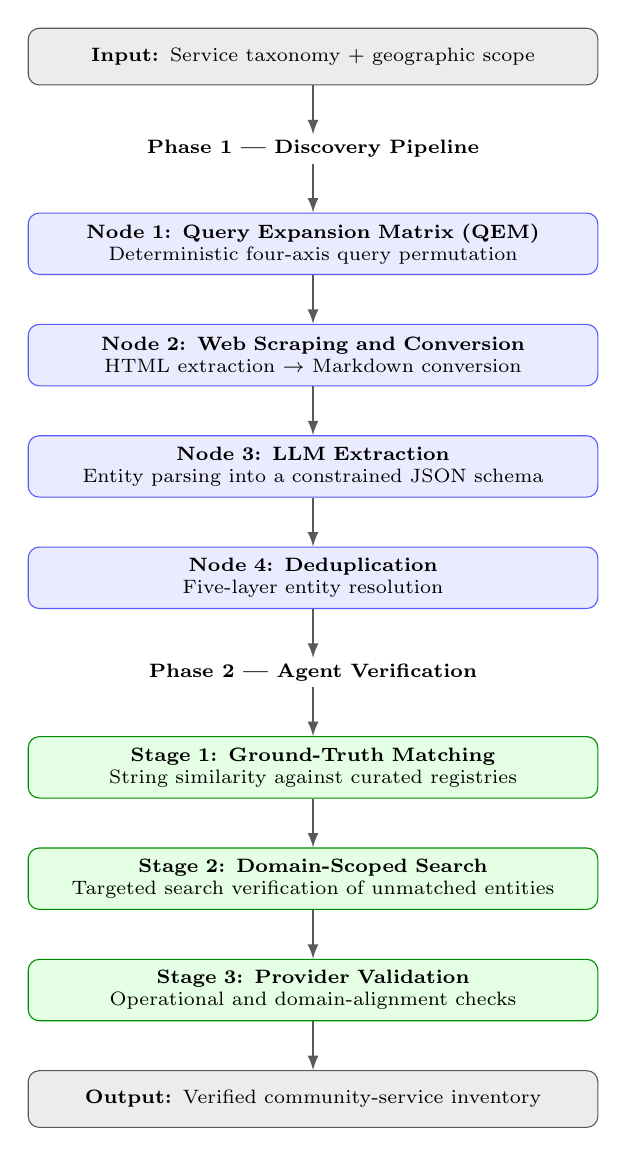
\begin{tikzpicture}[
	scale=1.0, transform shape,
	node distance=0.62cm,
	process/.style={rectangle, rounded corners, draw=blue!65, fill=blue!8, text width=7.0cm, minimum height=0.78cm, align=center, font=\scriptsize},
	phase/.style={font=\scriptsize\bfseries, align=center, draw=none, fill=none, inner sep=2pt},
	verify/.style={rectangle, rounded corners, draw=green!55!black, fill=green!10, text width=7.0cm, minimum height=0.78cm, align=center, font=\scriptsize},
	io/.style={rectangle, rounded corners, draw=black!65, fill=gray!15, text width=7.0cm, minimum height=0.72cm, align=center, font=\scriptsize},
	arrow/.style={-latex, thick, draw=black!65}
]
\node (input) [io] {\textbf{Input:} Service taxonomy + geographic scope};
\node (phase1) [phase, below=of input] {Phase 1 --- Discovery Pipeline};
\node (qem) [process, below=of phase1] {\textbf{Node 1: Query Expansion Matrix (QEM)}\\Deterministic four-axis query permutation};
\node (scrape) [process, below=of qem] {\textbf{Node 2: Web Scraping and Conversion}\\HTML extraction $\rightarrow$ Markdown conversion};
\node (extract) [process, below=of scrape] {\textbf{Node 3: LLM Extraction}\\Entity parsing into a constrained JSON schema};
\node (dedup) [process, below=of extract] {\textbf{Node 4: Deduplication}\\Five-layer entity resolution};
\node (phase2) [phase, below=of dedup] {Phase 2 --- Agent Verification};
\node (match) [verify, below=of phase2] {\textbf{Stage 1: Ground-Truth Matching}\\String similarity against curated registries};
\node (search) [verify, below=of match] {\textbf{Stage 2: Domain-Scoped Search}\\Targeted search verification of unmatched entities};
\node (api) [verify, below=of search] {\textbf{Stage 3: Provider Validation}\\Operational and domain-alignment checks};
\node (output) [io, below=of api, node distance=0.8cm] {\textbf{Output:} Verified community-service inventory};
\draw [arrow] (input) -- (phase1);
\draw [arrow] (phase1) -- (qem);
\draw [arrow] (qem) -- (scrape);
\draw [arrow] (scrape) -- (extract);
\draw [arrow] (extract) -- (dedup);
\draw [arrow] (dedup) -- (phase2);
\draw [arrow] (phase2) -- (match);
\draw [arrow] (match) -- (search);
\draw [arrow] (search) -- (api);
\draw [arrow] (api) -- (output);
\end{tikzpicture}
\caption{ARS discovery and verification pipeline adapted from thesis Figure 3.1. The vertical layout retains the full sequence of discovery, extraction, entity resolution, and evidence-verification stages.}
\label{fig:journal_ars_pipeline}
\end{figure}

\subsection{Pathways Maintenance Layer}

Pathways converts the verified inventory into a searchable projection backed by an event-sourced ledger. The ledger stores immutable events such as field verification, issue reports, restoration requests, and accepted corrections. Current resource state is derived from those events rather than replacing the historical record. This design preserves chain of custody and allows the system to distinguish a value’s current display state from the evidence and interactions that produced it.

The user workflow follows four connected phases, shown in Figure~\ref{fig:journal_pathways_flywheel}. In \textit{Find}, structured filters and resource evidence are used to present candidate services. In \textit{Verify}, a navigator confirms individual fields when the information appears current. In \textit{Ask}, a stale or missing field becomes a structured restoration request that can be enriched by the ARS. In \textit{Close}, a human operator reviews the proposed value and accepts, rejects, or leaves it unresolved. Each action becomes an event that can update the derived projection while retaining the prior state.

\begin{figure}[H]
\centering
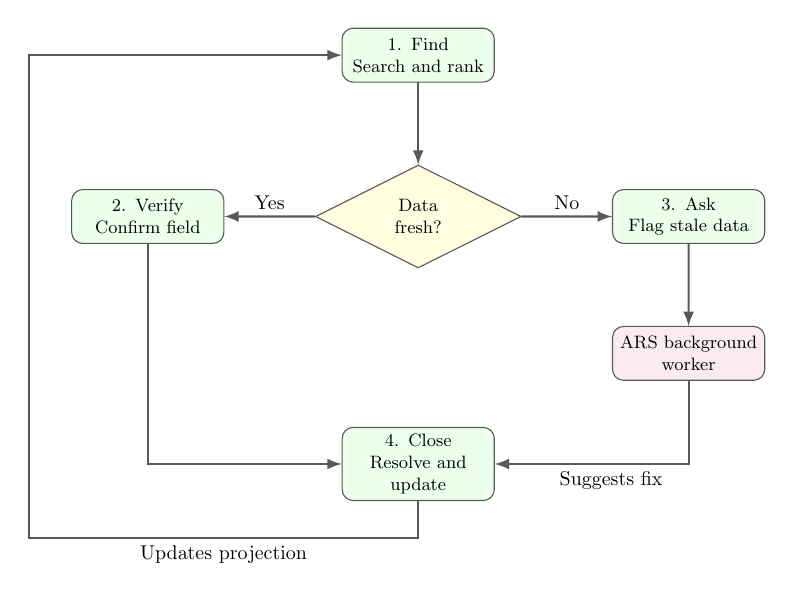
\begin{tikzpicture}[
	scale=0.72, transform shape,
	node distance=1.45cm and 1.6cm,
	process/.style={rectangle, rounded corners, draw=black!65, fill=green!8, text width=2.45cm, minimum height=0.95cm, align=center, font=\small},
	decision/.style={diamond, aspect=2, draw=black!65, fill=yellow!12, text width=2.0cm, align=center, inner sep=2pt, font=\small},
	worker/.style={rectangle, rounded corners, draw=black!65, fill=purple!8, text width=2.45cm, minimum height=0.95cm, align=center, font=\small},
	arrow/.style={-latex, thick, draw=black!65}
]
\node (find) [process] {1. Find\\Search and rank};
\node (fresh) [decision, below=of find] {Data\\fresh?};
\node (verify) [process, left=of fresh] {2. Verify\\Confirm field};
\node (ask) [process, right=of fresh] {3. Ask\\Flag stale data};
\node (worker) [worker, below=of ask] {ARS background\\worker};
\node (close) [process, below=of fresh, yshift=-1.35cm] {4. Close\\Resolve and update};
\draw [arrow] (find) -- (fresh);
\draw [arrow] (fresh) -- node[above] {Yes} (verify);
\draw [arrow] (fresh) -- node[above] {No} (ask);
\draw [arrow] (ask) -- (worker);
\draw [arrow] (worker) |- node[below, pos=0.7] {Suggests fix} (close.east);
\draw [arrow] (verify) |- (close.west);
\draw [arrow] (close.south) -- ++(0,-0.65cm) -| node[pos=0.25, below] {Updates projection} ([xshift=-0.75cm]verify.west) |- (find.west);
\end{tikzpicture}
\caption{Pathways Find--Verify--Ask--Close flywheel adapted from thesis Figure 4.7. Human validation updates the derived projection, while stale-field requests delegate restoration to the ARS.}
\label{fig:journal_pathways_flywheel}
\end{figure}

\subsection{Integrated Evidence Flow}

The two figures show how the system moves from broad discovery to accountable maintenance. ARS broadens the candidate space and proposes structured values; Pathways makes provenance visible and reserves acceptance decisions for evidence-backed review. This creates a common contract between the systems: every restored value must identify its target organization, requested field, supporting source, and adjudication status. The contract supports reproducible evaluation and allows unresolved or weakly supported values to remain visible as review work instead of being presented as verified facts.

%%%%%%%%%%%%%%%%%%%%%%%%%%%%%%%%%%%%%%%%%%
\section{Materials and Methods}

\subsection{Study Design}

The evaluation was designed to test two distinct capabilities of the integrated system. Study 1 measures whether free-text requests are translated into the structured filters consumed by Pathways search. Study 2 measures whether missing organizational fields can be restored with evidence sufficient for manual classification. The studies use separate fixtures and metrics because request interpretation and field restoration are different technical tasks.

\subsection{Study 1: Natural-Language Filter Extraction}

The Study 1 fixture contains 200 structured requests generated from ten filter families crossed with ten Ontario locations. Each family contributes one canonical request and one paraphrased request, producing 100 cases in each group. Gold labels cover seven fields used by Pathways: need, modality, population, coverage, location, language, and urgency.

Five extraction conditions isolate the contributions of the pipeline stages: basic deterministic rules, ontology aliases, semantic matching without language-model fallback, constrained Gemini fallback without the semantic stage, and semantic matching combined with constrained Gemini. The alias map and semantic phrase inventory are validated against the same ontology used to create the fixture; consequently, these results are treated as development-fixture evidence rather than held-out estimates of general language understanding.

The primary metric is exact-case accuracy, defined as the proportion of requests for which all seven output fields match the gold record. We also report field-level precision, recall, and micro-averaged F1. Gemini was used through the configured OpenAI-compatible endpoint with batched requests. Its output was restricted to permitted ontology values, and the fallback could abstain when no valid mapping was available.

\subsection{Study 2: Missing-Data Restoration}

Study 2 uses a sealed benchmark of 500 requested missing fields. The requested fields comprise 269 addresses, 112 phone numbers, 58 postal codes, and 61 websites. Each benchmark row provides the public organization and location context while withholding one target field. The sealed reference stores the expected value used for evaluation; the restoration workflow receives only the public row and provider- or web-derived evidence.

The workflow records whether a candidate was returned, whether it passed the entity-support check, and whether it matched the sealed value after field-specific normalization. Entity support combines name, city, address, postal code, and website-domain evidence. A candidate is not accepted solely because its value looks plausible; it must be associated with the intended organization under the matching rule. The final manual classification uses four outcomes: Exact, Supported, non-exact, Weakly supported, and Unresolved.

Supported, non-exact values include valid organizational representations such as departmental or branch phone numbers and alternate website pages. Weakly supported values are plausible but require confirmation, particularly when address granularity or postal-code assignment is uncertain. Unresolved values are empty, malformed, or rejected after review. A separate mismatch audit groups non-exact values by representation difference, likely alternate value, or need for verification. The audit also records extraction errors such as business-hours text or social-media URLs returned in response to a website request.

\subsection{Reproducibility and Data Governance}

The fixtures, evaluation reports, mismatch audit, and implementation scripts are retained with the project materials. The compact schemas and decision rules are summarized in Appendix~\ref{app:evaluation_protocol}. The benchmark concerns public organizational metadata rather than patient records or protected health information. The article reports the provenance and adjudication rules needed to reproduce the classifications while recognizing that third-party source data and provider APIs may change over time. No live clinical deployment or human-participant intervention was conducted in these studies.

\iffalse

The Materials and Methods should be described with sufficient detail to allow others to replicate and build on the published results. Please note that the publication of your manuscript implies that you must make all materials, data, computer code, and protocols associated with the publication available to readers. Please disclose at the submission stage any restrictions on the availability of materials or information. New methods and protocols should be described in detail while well-established methods can be briefly described and appropriately cited.

Research manuscripts reporting large datasets that are deposited in a publicly available database should specify where the data have been deposited and provide the relevant accession numbers. If the accession numbers have not yet been obtained at the time of submission, please state that they will be provided during review. They must be provided prior to publication.

Interventionary studies involving animals or humans, and other studies that require ethical approval, must list the authority that provided approval and the corresponding ethical approval code.

In this section, where applicable, authors are required to disclose details of how generative artificial intelligence (GenAI) has been used in this paper (e.g., to generate text, data, or graphics, or to assist in study design, data collection, analysis, or interpretation). The use of GenAI for superficial text editing (e.g., grammar, spelling, punctuation, and formatting) does not need to be declared.

\begin{quote}
This is an example of a quote.
\end{quote}

%%%%%%%%%%%%%%%%%%%%%%%%%%%%%%%%%%%%%%%%%%
\section{Results}

This section may be divided by subheadings. It should provide a concise and precise description of the experimental results, their interpretation, and the experimental conclusions that can be drawn.

\subsection{Subsection}
\subsubsection{Subsubsection}

Bulleted lists look like this:
\begin{itemize}
\item	First bullet;
\item	Second bullet;
\item	Third bullet.
\end{itemize}

Numbered lists can be added as follows:
\begin{enumerate}
\item	First item; 
\item	Second item;
\item	Third item.
\end{enumerate}

The text continues here.

\subsection{Figures, Tables and Schemes}

All figures and tables should be cited in the main text as Figure~\ref{fig1}, Table~\ref{tab1}, etc.

\begin{figure}[H]
%\isPreprints{\centering}{} % Only used for preprints

\includegraphics[width=8.0 cm]{Definitions/logo-mdpi}
\caption{This is a figure. Schemes follow the same formatting.\label{fig1}}
\end{figure}   
\unskip

\begin{table}[H] 
%\small % Change table font size
\caption{This is a table caption. Tables should be placed in the main text near the first time they are~cited.\label{tab1}}
%\isPreprints{\centering}{} % Only used for preprints
\begin{tabularx}{\textwidth}{CCC}
\toprule
\textbf{Title 1}	& \textbf{Title 2}	& \textbf{Title 3}\\
\midrule
Entry 1		& Data			& Data\\
Entry 2		& Data			& Data \textsuperscript{1}\\
\bottomrule
\end{tabularx}

\noindent{\small{\textsuperscript{1} Tables may have a footer.}}
\end{table}

The text continues here (Figure~\ref{fig2} and Table~\ref{tab2}).

% Example of a figure that spans the whole page width and with subfigures. The same concept works for tables, too.
\begin{figure}[H]
%\isPreprints{}{% This command is only used for ``preprints''.
\begin{adjustwidth}{-\extralength}{0cm}
\centering
%} % If the paper is ``preprints'', please uncomment this parenthesis.
\subfloat[\centering]{
\includegraphics[width=7.0cm]{Definitions/logo-mdpi}}
%\hfill
\subfloat[\centering]{
\includegraphics[width=7.0cm]{Definitions/logo-mdpi}}\\
\subfloat[\centering]{
\includegraphics[width=7.0cm]{Definitions/logo-mdpi}}
%\hfill
\subfloat[\centering]{
\includegraphics[width=7.0cm]{Definitions/logo-mdpi}}
%\isPreprints{}{% This command is only used for ``preprints''.
\end{adjustwidth}
%} % If the paper is ``preprints'', please uncomment this parenthesis.
\caption{This is a wide figure. Schemes follow the same formatting. If there are multiple panels, they should be listed as follows: (\textbf{a}) Description of what is contained in the first panel. (\textbf{b}) Description of what is contained in the second panel. (\textbf{c}) Description of what is contained in the third panel. (\textbf{d}) Description of what is contained in the fourth panel. Figures should be placed in the main text near the first time they are cited.\label{fig2}}
\end{figure} 

\begin{table}[H]
\caption{This is a wide table. Tables should be placed in the main text near the first time they are~cited.\label{tab2}}
%\isPreprints{\centering}{% This command is only used for ``preprints''.
	\begin{adjustwidth}{-\extralength}{0cm}
%} % If the paper is ``preprints'', please uncomment this parenthesis.
%\isPreprints{\begin{tabularx}{\textwidth}{CCCC}}{% This command is only used for ``preprints''.
		\begin{tabularx}{\fulllength}{CCCC}
%} % If the paper is ``preprints'', please uncomment this parenthesis.
			\toprule
			\textbf{Title 1}	& \textbf{Title 2}	& \textbf{Title 3}     & \textbf{Title 4}\\
			\midrule
\multirow[m]{3}{*}{Entry 1 *}	& Data			& Data			& Data\\
			  	                   & Data			& Data			& Data\\
			             	      & Data			& Data			& Data\\
                   \midrule
\multirow[m]{3}{*}{Entry 2}    & Data			& Data			& Data\\
			  	                  & Data			& Data			& Data\\
			             	     & Data			& Data			& Data\\
			\bottomrule
		\end{tabularx}
%		\isPreprints{}{% This command is only used for ``preprints''.
	\end{adjustwidth}
%} % If the paper is ``preprints'', please uncomment this parenthesis.
	\noindent{\small{* Tables may have a footer.}}
\end{table}

%\begin{listing}[H]
%\caption{Title of the listing}
%\rule{\columnwidth}{1pt}
%\raggedright Text of the listing. In font size footnotesize, small, or normalsize. Preferred format: left aligned and single spaced. Preferred border format: top border line and bottom border line.
%\rule{\columnwidth}{1pt}
%\end{listing}

Text.

Text.

\subsection{Formatting of Mathematical Components}

This is example 1 of an equation:
\begin{equation}
a = 1,
\end{equation}
the text following an equation need not be a new paragraph if it continues a sentence. Please punctuate equations as regular text.

This is example 2 of an equation:
%\isPreprints{}{% This command is only used for ``preprints''.
\begin{adjustwidth}{-\extralength}{0cm}
%} % If the paper is ``preprints'', please uncomment this parenthesis.
\begin{equation}
a = b + c + d + e + f + g + h + i + j + k + l + m + n + o + p + q + r + s + t + u + v + w + x + y + z
\end{equation}
%\isPreprints{}{% This command is only used for ``preprints''.
\end{adjustwidth}
%} % If the paper is ``preprints'', please uncomment this parenthesis.

If the text following an equation starts a new sentence, it should be a new paragraph. Please punctuate equations as regular text.

%% Example of a page in landscape format (with table and table footnote).
%\startlandscape
%\begin{table}[H] %% Table in wide page
%%\isPreprints{\centering}{} % This command is only used for ``preprints''.
%\caption{This is a very wide table.\label{tab3}}
%	\begin{tabularx}{\textwidth}{CCCC}
%		\toprule
%		\textbf{Title 1}	& \textbf{Title 2}	& \textbf{Title 3}	& \textbf{Title 4}\\
%		\midrule
%		Entry 1		& Data			& Data			& This cell has some longer content that runs over two lines.\\
%		Entry 2		& Data			& Data			& Data\textsuperscript{1}\\
%		\bottomrule
%	\end{tabularx}
%%\isPreprints{}{% This command is only used for ``preprints''.
%	\begin{adjustwidth}{+\extralength}{0cm}
%%} % If the paper is ``preprints'', please uncomment this parenthesis.
%		\noindent\small{\textsuperscript{1} This is a table footnote.}
%%\isPreprints{}{% This command is only used for ``preprints''.
%	\end{adjustwidth}
%%} % If the paper is ``preprints'', please uncomment this parenthesis.
%\end{table}
%\finishlandscape

Theorem-type environments (including propositions, lemmas, corollaries, etc.) can be formatted as follows:
%% Example of a theorem:
\begin{Theorem}
Example text of a theorem. Theorems, propositions, lemmas, etc., should be numbered sequentially (i.e., Proposition 2 follows Theorem 1). Examples or Remarks use the same formatting, but should be numbered separately, so a document may contain Theorem 1, Remark 1 and Example~1.
\end{Theorem}

The text continues here. Proofs must be formatted as follows:

%% Example of a proof:
\begin{proof}[Proof of Theorem 1]
Text of the proof. Note that the phrase ``of Theorem 1'' is optional if it is clear which theorem is being referred to.
\end{proof}
The text continues here.

%%%%%%%%%%%%%%%%%%%%%%%%%%%%%%%%%%%%%%%%%%
\fi

\section{Results}

\subsection{Study 1: Natural-Language Filter Extraction}

The extraction benchmark showed a clear progression as pipeline stages were added. Basic rules achieved 0.600 overall exact-case accuracy and 0.200 paraphrase accuracy. Ontology aliases improved paraphrase accuracy to 0.500, semantic matching to 0.800, and constrained Gemini fallback to 0.900. The combined semantic-plus-Gemini condition reached 1.000 on the development fixture. Because the fixture and ontology were used during implementation, these results demonstrate behavior on the tested cases rather than held-out generalization.

\begin{table}[H]
\caption{Study 1 filter-extraction results across five conditions.}
\label{tab:journal_study1}
\small
\begin{tabularx}{\textwidth}{@{}Xrrrr@{}}
\toprule
\textbf{Condition} & \textbf{Overall exact} & \textbf{Canonical exact} & \textbf{Paraphrased exact} & \textbf{Micro-F1} \\
\midrule
Basic rules & 0.600 & 1.000 & 0.200 & 0.8916 \\
Hybrid aliases & 0.750 & 1.000 & 0.500 & 0.9318 \\
Semantic-only & 0.900 & 1.000 & 0.800 & 0.9663 \\
Gemini-only & 0.950 & 1.000 & 0.900 & 0.9890 \\
Semantic + Gemini & 1.000 & 1.000 & 1.000 & 1.0000 \\
\bottomrule
\end{tabularx}
\end{table}

\begin{figure}[H]
\centering
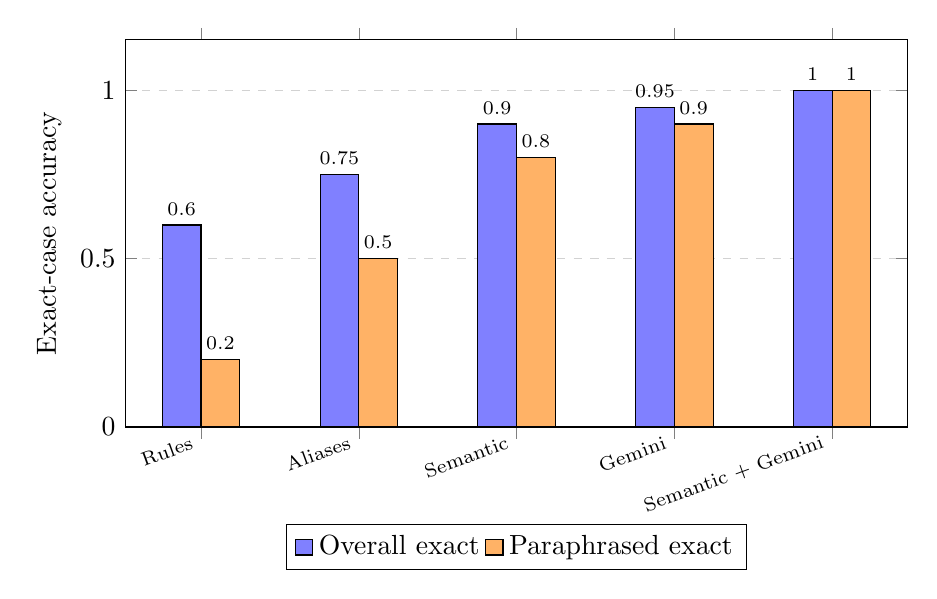
\begin{tikzpicture}
\begin{axis}[
	ybar, bar width=14pt, width=0.95\textwidth, height=6.5cm,
	ymin=0, ymax=1.15, ylabel={Exact-case accuracy},
	symbolic x coords={Rules,Aliases,Semantic,Gemini,Combined}, xtick=data,
	xticklabels={Rules,Aliases,Semantic,Gemini,Semantic + Gemini},
	x tick label style={font=\scriptsize, rotate=20, anchor=east},
	nodes near coords, nodes near coords style={font=\scriptsize},
	enlarge x limits=0.12, ymajorgrids=true, grid style={dashed,gray!35},
	legend style={at={(0.5,-0.25)},anchor=north,legend columns=2},
	legend image code/.code={\draw[#1,fill=#1] (0cm,-0.1cm) rectangle (0.22cm,0.1cm);}
]
\addplot[fill=blue!50, bar shift=-7pt] coordinates {(Rules,0.600) (Aliases,0.750) (Semantic,0.900) (Gemini,0.950) (Combined,1.000)};
\addlegendentry{Overall exact}
\addplot[fill=orange!60, bar shift=7pt] coordinates {(Rules,0.200) (Aliases,0.500) (Semantic,0.800) (Gemini,0.900) (Combined,1.000)};
\addlegendentry{Paraphrased exact}
\end{axis}
\end{tikzpicture}
\caption{Study 1 exact-case accuracy for overall and paraphrased requests.}
\label{fig:journal_study1}
\end{figure}

\subsection{Study 2: Missing-Data Restoration}

The restoration benchmark requested 500 missing fields. The workflow returned a candidate for 499 fields and all returned candidates passed the automated entity-support threshold. After manual review, 142 values were exact, 284 were supported but non-exact, 63 were weakly supported, and 11 were unresolved.

\begin{table}[H]
\caption{Study 2 restoration outcomes by missing-field category.}
\label{tab:journal_study2_fields}
\small
\begin{tabularx}{\textwidth}{@{}Xrrrrr@{}}
\toprule
\textbf{Missing field} & \textbf{Requested} & \textbf{Exact} & \textbf{Supported, non-exact} & \textbf{Weakly supported} & \textbf{Unresolved} \\
\midrule
Address & 269 & 11 & 201 & 57 & 0 \\
Phone number & 112 & 77 & 34 & 0 & 1 \\
Postal code & 58 & 52 & 0 & 6 & 0 \\
Website & 61 & 2 & 49 & 0 & 10 \\
\textbf{Total} & \textbf{500} & \textbf{142} & \textbf{284} & \textbf{63} & \textbf{11} \\
\bottomrule
\end{tabularx}
\end{table}

The benchmark was geographically concentrated in the Greater Toronto Area (GTA), which contributed 336 of 500 requested fields (67.2\%). All 11 unresolved fields occurred in the GTA. This pattern is reported as a descriptive property of the benchmark rather than evidence that restoration performance is uniformly different across regions.

\begin{table}[H]
\caption{Study 2 restoration outcomes by analytical region.}
\label{tab:journal_study2_geography}
\small
\begin{tabularx}{\textwidth}{@{}Xrrrrrr@{}}
\toprule
\textbf{Region} & \textbf{Requested} & \textbf{Share} & \textbf{Exact} & \textbf{Supported} & \textbf{Weak} & \textbf{Unresolved} \\
\midrule
GTA & 336 & 67.2\% & 131 & 159 & 35 & 11 \\
Northern Ontario & 48 & 9.6\% & 3 & 40 & 5 & 0 \\
Eastern Ontario & 42 & 8.4\% & 2 & 35 & 5 & 0 \\
Southwestern Ontario & 47 & 9.4\% & 4 & 32 & 11 & 0 \\
Central Ontario & 27 & 5.4\% & 2 & 18 & 7 & 0 \\
\textbf{Total} & \textbf{500} & \textbf{100.0\%} & \textbf{142} & \textbf{284} & \textbf{63} & \textbf{11} \\
\bottomrule
\end{tabularx}
\end{table}

The non-exact mismatch audit identified three broad causes: high-confidence representation differences (155 cases, 43.4\%), likely valid alternatives (75 cases, 21.0\%), and insufficient or ambiguous evidence (127 cases, 35.6\%). Address representation and granularity were the largest sources of review work. Website review also identified ten malformed outputs, including business-hours text and Facebook URLs returned for website requests; these were classified as unresolved rather than supported.

\begin{table}[H]
\caption{Study 2 quantitative audit of non-exact outcomes.}
\label{tab:journal_study2_root_causes}
\small
\begin{tabularx}{\textwidth}{@{}>{\raggedright\arraybackslash}Xrr>{\raggedright\arraybackslash}X>{\raggedright\arraybackslash}X@{}}
\toprule
\textbf{Cause group} & \textbf{Count} & \textbf{Share} & \textbf{Fields} & \textbf{Action} \\
\midrule
Format or representation & 155 & 43.4\% & Address, phone, website & Supported, non-exact \\
Likely alternate & 75 & 21.0\% & Address, phone & Supported or review \\
Needs verification & 127 & 35.6\% & Address, phone, postal, website & Manual review \\
\textbf{Total raw mismatches} & \textbf{357} & \textbf{100.0\%} & & \\
\bottomrule
\end{tabularx}
\end{table}

\section{Discussion}

The two evaluations support a bounded interpretation of the proposed architecture. In Study 1, each additional interpretation stage improved performance on paraphrased requests, with the combined semantic-plus-Gemini condition reaching perfect exact-case accuracy on the development fixture. This result supports the value of separating deterministic ontology handling from constrained language-model fallback. It does not establish open-ended language coverage because the query families and ontology were available during implementation.

Study 2 shows why missing-data restoration should not be reduced to exact string matching. Only 142 of 500 fields matched the sealed reference exactly, but a further 284 values were accepted as supported non-exact representations after review. These differences commonly reflected address wording, phone routing or extensions, and alternate organizational website representations. Treating every mismatch as a failure would underestimate useful recovery; treating every plausible candidate as correct would overstate reliability. The four-way classification makes that distinction explicit.

The root-cause audit further indicates that restoration quality depends on evidence management as much as retrieval. Representation differences and likely valid alternatives accounted for most non-exact cases, while 127 cases still required verification. The ten malformed website outputs demonstrate a separate extraction problem: a system can retrieve relevant page content while selecting the wrong field type. Provenance, field-specific validation, and human adjudication are therefore necessary safeguards for a directory intended to support care coordination.

The geographic breakdown provides important context for interpreting Study 2. The benchmark is concentrated in the GTA, and all unresolved cases occur there. This is a descriptive property of the sampled benchmark, not evidence that the system performs better in other regions. More geographically balanced fixtures and independent held-out organizations are needed before regional performance claims can be made.

Together, the results support Pathways as an auditable assistive workflow. The system can broaden interpretation and recover useful organizational information, but it should not be treated as an autonomous source of truth. The architecture’s contribution is the combination of deterministic coverage, constrained interpretation, evidence provenance, and explicit human review.

\section{Limitations}

Several limitations qualify these findings. First, Study 1 is a development-fixture evaluation: the ontology, query families, and paraphrase construction were available during implementation. A held-out benchmark created independently of the extraction rules is required to estimate generalization.

Second, Study 2 combines automated entity support with manual adjudication. The outcome labels are reproducible under the stated rules, but some organizational representations remain judgment-dependent. The sealed references also represent one source convention and may not always be the only valid current value.

Third, the restoration benchmark is geographically imbalanced and concerns public organizational metadata rather than live clinical referral outcomes. It does not measure user adoption, referral success, clinical workload, or longitudinal freshness in a deployed health network. The present work also relies on external web and provider evidence that can change over time or be unavailable for organizations with limited digital presence.

Finally, the system was evaluated as an integrated prototype rather than through a randomized live deployment. Future work should use independent fixtures, broader geographic sampling, controlled ontology expansion, source archiving, and prospective evaluation with clinical navigators.

%%%%%%%%%%%%%%%%%%%%%%%%%%%%%%%%%%%%%%%%%%
\section{Conclusions}

The proposed pipeline combines deterministic long-tail search construction with constrained extraction, evidence-backed restoration, and human-mediated maintenance. Across the two development evaluations, it improved paraphrase interpretation and recovered 499 candidate values, of which 426 were classified as exact or supported non-exact after review. These results support further investigation of auditable AI-assisted directory maintenance while preserving a clear boundary between useful assistance and verified clinical authority.

%%%%%%%%%%%%%%%%%%%%%%%%%%%%%%%%%%%%%%%%%%
\vspace{6pt} 

%%%%%%%%%%%%%%%%%%%%%%%%%%%%%%%%%%%%%%%%%%
%% optional
%\supplementary{The following supporting information can be downloaded at \linksupplementary{s1}, Figure S1: title; Table S1: title; Video S1: title.}

% Only for journal Methods and Protocols:
% If you wish to submit a video article, please do so with any other supplementary material.
% \supplementary{The following supporting information can be downloaded at \linksupplementary{s1}, Figure S1: title; Table S1: title; Video S1: title. A supporting video article is available at doi: link.}

% Only used for preprtints:
% \supplementary{The following supporting information can be downloaded at the website of this paper posted on \href{https://www.preprints.org/}{Preprints.org}.}

% Only for journal Hardware:
% If you wish to submit a video article, please do so with any other supplementary material.
% \supplementary{The following supporting information can be downloaded at \linksupplementary{s1}, Figure S1: title; Table S1: title; Video S1: title.\vspace{6pt}\\
%\begin{tabularx}{\textwidth}{lll}
%\toprule
%\textbf{Name} & \textbf{Type} & \textbf{Description} \\
%\midrule
%S1 & Python script (.py) & Script of python source code used in XX \\
%S2 & Text (.txt) & Script of modelling code used to make Figure X \\
%S3 & Text (.txt) & Raw data from experiment X \\
%S4 & Video (.mp4) & Video demonstrating the hardware in use \\
%... & ... & ... \\
%\bottomrule
%\end{tabularx}
%}

%%%%%%%%%%%%%%%%%%%%%%%%%%%%%%%%%%%%%%%%%%
\authorcontributions{Conceptualization, Kevin Igweh, Ajmery Sultana and Randy Lin; methodology, Kevin Igweh; software, Kevin Igweh; validation, Kevin Igweh, Ajmery Sultana and Randy Lin; formal analysis, Kevin Igweh; investigation, Kevin Igweh; data curation, Kevin Igweh; writing---original draft preparation, Kevin Igweh; writing---review and editing, Kevin Igweh, Ajmery Sultana, Randy Lin and Teryn Bruni; visualization, Kevin Igweh; supervision, Ajmery Sultana and Randy Lin; project administration, Kevin Igweh. All authors have read and agreed to the published version of the manuscript.}

\funding{This research received no external funding.}

\institutionalreview{Not applicable. The studies analyzed public organizational metadata and did not involve human participants, patient records, or animal subjects.}

\informedconsent{Not applicable. The studies did not involve human participants or identifiable personal data.}

\dataavailability{The study fixtures, evaluation reports, mismatch audit, and analysis scripts are available from the corresponding author on reasonable request. The benchmark uses public organizational metadata and provider-derived evidence; source availability may change over time and third-party datasets remain subject to their original access conditions.}

%\durcstatement{Current research is limited to the [please insert a specific academic field, e.g., XXX], which is beneficial [share benefits and/or primary use] and does not pose a threat to public health or national security. Authors acknowledge the dual-use potential of the research involving xxx and confirm that all necessary precautions have been taken to prevent potential misuse. As an ethical responsibility, authors strictly adhere to relevant national and international laws about DURC. Authors advocate for responsible deployment, ethical considerations, regulatory compliance, and transparent reporting to mitigate misuse risks and foster beneficial outcomes.}

% Only for journal Nursing Reports
%\publicinvolvement{Please describe how the public (patients, consumers, carers) were involved in the research. Consider reporting against the GRIPP2 (Guidance for Reporting Involvement of Patients and the Public) checklist. If the public were not involved in any aspect of the research add: ``No public involvement in any aspect of this research''.}
%
%% Only for journal Nursing Reports
%\guidelinesstandards{Please add a statement indicating which reporting guideline was used when drafting the report. For example, ``This manuscript was drafted against the XXX (the full name of reporting guidelines and citation) for XXX (type of research) research''. A complete list of reporting guidelines can be accessed via the equator network: \url{https://www.equator-network.org/}.}
%
%% Only for journal Nursing Reports
%\useofartificialintelligence{Please describe in detail any and all uses of artificial intelligence (AI) or AI-assisted tools used in the preparation of the manuscript. This may include, but is not limited to, language translation, language editing and grammar, or generating text. Alternatively, please state that “AI or AI-assisted tools were not used in drafting any aspect of this manuscript”.}

\acknowledgments{The authors acknowledge Algoma University for supporting the research environment. During preparation of this manuscript, the authors used GitHub Copilot for drafting assistance, language editing, and formatting support. The authors reviewed and edited all generated material and take full responsibility for the content of this publication.}

\conflictsofinterest{The authors declare no conflicts of interest.}

%%%%%%%%%%%%%%%%%%%%%%%%%%%%%%%%%%%%%%%%%%
%% Optional

%% Only for journal Encyclopedia
%\entrylink{The Link to this entry published on the encyclopedia platform.}

\abbreviations{Abbreviations}{%
The following abbreviations are used in this manuscript:\\

\noindent 
\begin{tabular}{@{}ll}
ARS & Agentic Research System\\
QEM & Query Expansion Matrix\\
LLM & Large Language Model\\
SDoH & Social Determinants of Health
\end{tabular}
}

%%%%%%%%%%%%%%%%%%%%%%%%%%%%%%%%%%%%%%%%%%
%% Optional
\appendixtitles{yes}
\appendixstart
\appendix
\section{Evaluation Protocol Details}\label{app:evaluation_protocol}

This appendix records the compact decision schema used by the two evaluations. The full fixtures, raw reports, mismatch audit, and execution scripts are retained as research materials rather than reproduced here.

\subsection{Study 1 Schema and Conditions}
\begin{table}[H]
\caption{Study 1 structured filter schema.}
\label{tab:appendix_study1_schema}
\small
\begin{tabularx}{\textwidth}{@{}p{2.3cm}X@{}}
\toprule
\textbf{Field} & \textbf{Purpose} \\
\midrule
Need & Target service or problem area. \\
Modality & Delivery mode, such as in-person or remote. \\
Population & Intended population or age group. \\
Coverage & Eligibility or payment coverage. \\
Location & Municipality or geographic area. \\
Language & Requested service language. \\
Urgency & Timing requirement, such as same-day service. \\
\bottomrule
\end{tabularx}
\end{table}

The 200-query fixture contains ten filter families crossed with ten Ontario locations. Each family contributes one canonical and one paraphrased request. The evaluated conditions are: (i) basic deterministic rules; (ii) rules plus ontology aliases; (iii) semantic matching without language-model fallback; (iv) constrained Gemini fallback without semantic matching; and (v) semantic matching combined with constrained Gemini. Exact-case accuracy requires all seven fields to match the gold record.

\subsection{Study 2 Classification Rules}
\begin{table}[H]
\caption{Study 2 field-outcome definitions.}
\label{tab:appendix_study2_outcomes}
\small
\begin{tabularx}{\textwidth}{@{}p{3.0cm}X@{}}
\toprule
\textbf{Outcome} & \textbf{Decision rule} \\
\midrule
Exact & Candidate matches the sealed reference after field-specific normalization. \\
Supported, non-exact & Candidate differs from the reference but manual evidence supports it as a valid value for the intended organization. \\
Weakly supported & Candidate is plausible or related but requires additional confirmation before acceptance. \\
Unresolved & No usable value was returned, or the candidate was malformed or rejected during review. \\
\bottomrule
\end{tabularx}
\end{table}

Automated entity support combines agreement across organization name, city, address, postal code, and website domain. The mismatch audit then groups non-exact values into representation differences, likely valid alternatives, and cases requiring verification. Website outputs containing business-hours text or unsuitable social-media URLs are treated as extraction errors and remain unresolved.

\iffalse
\appendixtitles{no} % Leave argument "no" if all appendix headings stay EMPTY (then no dot is printed after "Appendix A"). If the appendix sections contain a heading then change the argument to "yes".
\appendixstart
\appendix
\section[\appendixname~\thesection]{}
\subsection[\appendixname~\thesubsection]{}

The appendix is an optional section that can contain details and data supplemental to the main text---for example, explanations of experimental details that would disrupt the flow of the main text but nonetheless remain crucial to understanding and reproducing the research shown; figures of replicates for experiments of which representative data are shown in the main text can be added here if brief, or as Supplementary Materials. Mathematical proofs of results not central to the paper can be added as an appendix.

\begin{table}[H] 
\caption{This is a table caption.\label{tab5}}
%\newcolumntype{C}{>{\centering\arraybackslash}X}
\begin{tabularx}{\textwidth}{CCC}
\toprule
\textbf{Title 1}	& \textbf{Title 2}	& \textbf{Title 3}\\
\midrule
Entry 1		& Data			& Data\\
Entry 2		& Data			& Data\\
\bottomrule
\end{tabularx}
\end{table}

\section[\appendixname~\thesection]{}

All appendix sections must be cited in the main text. In the appendices, figures, tables, etc., should be labeled starting with “A”, e.g., Figure A1, Figure A2, etc.
\fi

%%%%%%%%%%%%%%%%%%%%%%%%%%%%%%%%%%%%%%%%%%
%\isPreprints{}{% This command is only used for ``preprints''.
\clearpage
\begin{adjustwidth}{-\extralength}{0cm}
%} % If the paper is ``preprints'', please uncomment this parenthesis.
%\printendnotes[custom] % Un-comment to print a list of endnotes

\reftitle{References}

% References must be numbered in order of appearance in the text (including citations in tables and legends) and listed individually at the end of the manuscript. We recommend preparing the references with a bibliography software package, such as EndNote, ReferenceManager or Zotero, to avoid typing mistakes and duplicated references. Include the digital object identifier (DOI) for all references where available.
% Please provide either the correct journal abbreviation (e.g. according to the “The list of Title Word Abbreviations” https://portal.issn.org/ltwa) or the full name of the journal. 
% Citations and references in the Supplementary Materials are permitted provided that they also appear in the reference list here. 
% In the text, reference numbers should be placed in square brackets [ ] and placed before the punctuation; for example, [1], [1–3] or [1,3]. For embedded citations in the text with pagination, use both parentheses and brackets to indicate the reference number and page numbers; for example, [5] (p. 10), or [6] (pp. 101–105).

%=====================================
% References, variant A: external bibliography
%=====================================
% \bibliography{your_external_BibTeX_file}

%=====================================
% References, variant B: internal bibliography
%=====================================

% ACS format
\begin{thebibliography}{999}
\bibitem{nakano2021webgpt}
Nakano, R.; Hilton, J.; Stoica, I.; et al. WebGPT: Browser-Assisted Question-Answering with Human Feedback. In \textit{Advances in Neural Information Processing Systems}; 2021.

\bibitem{zhou2024webarena}
Zhou, Y.; et al. WebArena: A Realistic Web Environment for Building Autonomous Agents. In \textit{International Conference on Learning Representations}; 2024.

\bibitem{yao2023react}
Yao, S.; Zhao, J.; Yu, D.; et al. ReAct: Synergizing Reasoning and Acting in Language Models. In \textit{International Conference on Learning Representations}; 2023.

\bibitem{khao2023seo}
Khao, A.; et al. Agentic Search and the SEO Trap in Generative Models. \textit{Journal of Artificial Intelligence Research} \textbf{2023}.

\bibitem{abdulnazar2024}
Abdulnazar, A.; et al. Large Language Models for Clinical Text Cleansing Enhance Medical Concept Normalization. \textit{IEEE Access} \textbf{2024}.

\bibitem{ji2023hallucination}
Ji, Z.; et al. Survey of Hallucination in Natural Language Generation. \textit{ACM Computing Surveys} \textbf{2023}, \textit{55}.

\bibitem{lewis2020rag}
Lewis, P.; et al. Retrieval-Augmented Generation for Knowledge-Intensive NLP Tasks. In \textit{Advances in Neural Information Processing Systems}; 2020.

\bibitem{amershi2014}
Amershi, S.; et al. Power to the People: The Role of Humans in Interactive Machine Learning. \textit{AI Magazine} \textbf{2014}, \textit{35}.

\bibitem{olawade2026human}
Olawade, D.B.; et al. Human-in-the-Loop Artificial Intelligence in Healthcare: Applications, Outcomes, and Implementation Challenges. \textit{International Journal of Medical Informatics} \textbf{2026}, \textit{213}, 106362.

\bibitem{toolformer2023}
Schick, T.; et al. Toolformer: Language Models Can Teach Themselves to Use Tools. \textit{Advances in Neural Information Processing Systems} \textbf{2023}.

\bibitem{gorilla2023}
Patil, S.G.; et al. Gorilla: Large Language Model Connected with Massive APIs. \textit{arXiv} \textbf{2023}, arXiv:2305.15334.

\bibitem{toolllm2023}
Qin, Y.; et al. ToolLLM: Facilitating Large Language Models to Master 16000+ Real-World APIs. \textit{arXiv} \textbf{2023}, arXiv:2307.16789.

\bibitem{webvoyager2024}
He, H.; et al. WebVoyager: Building an End-to-End Web Agent with Large Multimodal Models. \textit{arXiv} \textbf{2024}, arXiv:2401.13919.

\bibitem{autogen2023}
Wu, Q.; et al. AutoGen: Enabling Next-Gen LLM Applications via Multi-Agent Conversation. In \textit{International Conference on Learning Representations}; 2023.

\bibitem{babyagi2023}
Richards, Y. BabyAGI: Task-Driven Autonomous Agent. GitHub Repository, 2023.

\bibitem{deepresearch2025}
OpenAI. Introducing Deep Research. OpenAI Research Blog, 2025.

\bibitem{gemini2024}
Google DeepMind. Gemini 1.5: Unlocking Multimodal Understanding across Millions of Tokens of Context. \textit{arXiv} \textbf{2024}, arXiv:2403.05530.

\bibitem{claude2024}
Anthropic. Developing a Computer Use Model. Anthropic News, 2024.

\bibitem{qiu2020}
Qiu, X.; et al. Pre-Trained Models for Natural Language Processing: A Survey. \textit{Science China Technological Sciences} \textbf{2020}, \textit{63}.

\bibitem{lample2016}
Lample, G.; et al. Neural Architectures for Named Entity Recognition. In \textit{Proceedings of NAACL}; 2016.

\bibitem{healthcare_survey2025}
He, K.; et al. A Survey of Large Language Models for Healthcare: From Data, Technology, and Applications to Accountability and Ethics. \textit{arXiv} \textbf{2025}, arXiv:2310.05694.

\bibitem{llm_survey2023}
Zhao, W.X.; et al. A Survey of Large Language Models. \textit{arXiv} \textbf{2023}, arXiv:2303.18223.

\bibitem{gero2023}
Gero, Z.; et al. Self-Verification Improves Few-Shot Clinical Information Extraction. \textit{arXiv} \textbf{2023}, arXiv:2306.00024.

\bibitem{dhuliawala2023}
Dhuliawala, S.; et al. Chain-of-Verification Reduces Hallucination in Large Language Models. \textit{arXiv} \textbf{2023}, arXiv:2309.11495.

\bibitem{fowler_event}
Fowler, M. Event Sourcing. Martin Fowler. Available online: \url{https://martinfowler.com/eaaDev/EventSourcing.html} (accessed on 2 October 2026).

\end{thebibliography}

% If authors have biography, please use the format below
%\section*{Short Biography of Authors}
%\bio
%{\raisebox{-0.35cm}{\includegraphics[width=3.5cm,height=5.3cm,clip,keepaspectratio]{Definitions/author1.pdf}}}
%{\textbf{Firstname Lastname} Biography of first author}
%
%\bio
%{\raisebox{-0.35cm}{\includegraphics[width=3.5cm,height=5.3cm,clip,keepaspectratio]{Definitions/author2.jpg}}}
%{\textbf{Firstname Lastname} Biography of second author}

%%%%%%%%%%%%%%%%%%%%%%%%%%%%%%%%%%%%%%%%%%
%% for journal Sci
%\reviewreports{\\
%Reviewer 1 comments and authors’ response\\
%Reviewer 2 comments and authors’ response\\
%Reviewer 3 comments and authors’ response
%}
%%%%%%%%%%%%%%%%%%%%%%%%%%%%%%%%%%%%%%%%%%
\PublishersNote{}
%\isPreprints{}{% This command is only used for ``preprints''.
\end{adjustwidth}
%} % If the paper is ``preprints'', please uncomment this parenthesis.
\end{document}

